
\documentclass[12pt,handout]{beamer}
\usetheme{Copenhagen}
\usecolortheme{beaver}

\usepackage{color}
\usepackage[strings]{underscore}
\begin{document}

% \logo{
\includegraphics[height=0.5cm]{cet.jpg}} 

\title[{\bf ARIA}-Asterisk Radio Architecture]{{\bf A}sterisk {\bf R}ad{\bf I}o {\bf A}rchitecture}
\subtitle{\it VoIP Based Campus Announcement System}  
\author[Rajasree, Dhananjay, Abil, Deepak, Sujith, Thomas]{Prof:
  Rajasree M S.(Principal Investigator) \and Dhananjay M Balan \and Abil N Goerge \and
  Deepak Krishnan \and Thomas Abraham\and Sujith Ganapathiyil}
 
\institute[College Of Engineering] % (optional)
{
 
 
  Department Of Computer Science \& Engineering.\\
  College Of Engineering, Trivandrum\\
  University Of Kerala. \\
 
\centerline{
\includegraphics[height=1.0cm]{cet.jpg}}

}
\date{\today} 

\frame{\titlepage
  } 

\frame[plain]{\frametitle{Outline}\tableofcontents[currentframes]} 

\section{Introduction}
\subsection{Problem}

\frame{
  \frametitle{Problem}
  \bf{ \large A geographically large campus with many groups of students have to implement an announcement system.}

}

\frame{
  \frametitle{Conventional System}
  \begin{enumerate}
  \item {\bf No Flexibility} in selection of audience.\\
    {\it No way of communicating with a part of audience.}\pause
  \item Requires {\bf heavy cabling} around the campus. \pause
  \item Limited {\bf scalability and extensibility}.
    \begin{itemize}

    \item {\it System cannot grow beyond a point, power and
        load problems.}
    \item {\it No scope of extending the system
        further. (Things like video, two way paging
        etc.)} \pause
    \end{itemize}
    
\emph{\textcolor{red} {Use an existing network!!}}
  \end{enumerate}
}

\subsection{Approaches}

\frame{
  \frametitle{VoIP}
  {\it{\bf Voice Over Internet Protocol} is a family of technologies, methodologies, communication protocols, and transmission techniques for the delivery of voice communications and multimedia sessions over Internet Protocol (IP) networks, such as the Internet.}\\
  
  \hfill{\bf - Wikipedia.org, Accessed on February 1, 2012}
}

\subsection{VoIP Advantages}
\frame[shrink]{
  \frametitle{Advantages}
  \begin{enumerate}
\item Can utilize the existing IP network in campus. \\
    - A major cost in implementing the system can be made practically nil.\pause
  \item Each client can be addressed individually. \\
    - User can create groups to address on-the fly.\pause
  
  \item Scalable - Adding a new client is simple as long as there is
    network connectivity \\ 
    - No load problems. \pause
  \item Have an option to build advanced systems.\\
    - Video transmission.\\
    - Two way communication systems.
    \pause
  \item Provision for remote access. \pause
  \item Easy modification of system - No hard circuits.
  \end{enumerate}
}

\frame{   
  \frametitle{Products Currently Available}

  \begin{enumerate}
  \item LanTone Systems. - \url{http://www.voip.com.sg/voip-products/ip-pa-system.html}
  \item AbleTEK IP-PA System - 
      \url{http://www.abletek.co.uk/ip\_public\_address.php}
  \item TalkMaster System - \url{http://www.digac.com/ii3\_talkmaster.htm}
  \end{enumerate} \pause
  All these products cost {\bf \~\$1500} for the software itself, and comes
  with a minimum {\bf device purchase limit} and {\bf no inter-operability}.\pause
 
  {\bf No Free Software} products exist, Though almost all core components are available in a compatible license   
}

\section{ARIA System.}
\frame{
\frametitle{ARIA}
  \large{\bf A}sterisk {\bf R}ad{\bf I}o {\bf A}rchitecture
}

\subsection{Design}

\frame{
  \frametitle{Block Diagram}
  \centerline{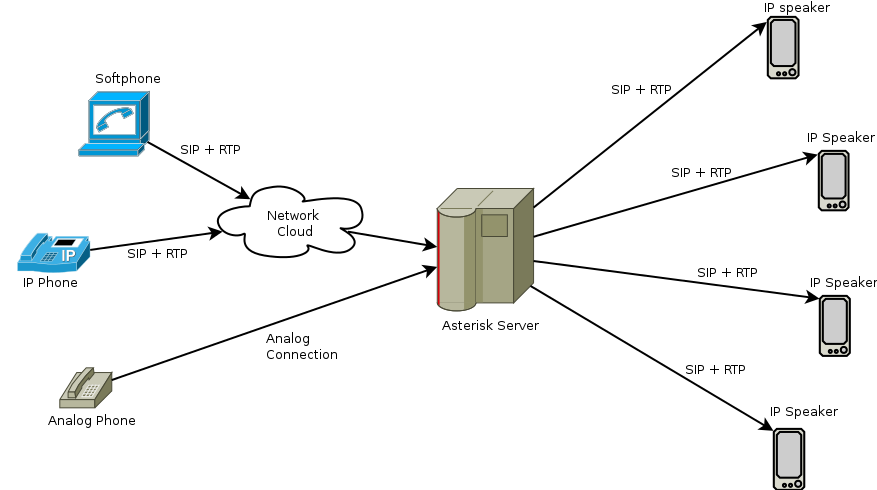
\includegraphics[width=\textwidth]{functional_diagram.png}}
}

\subsection{ARIA-Components}
\frame{
  \frametitle{Protocols}
  \begin{enumerate}
  \item The {\bf Session Initiation Protocol (SIP)} is an IETF-defined signaling protocol widely used for controlling communication sessions such as voice and video calls over Internet Protocol (IP). The protocol can be used for creating, modifying and terminating two-party (unicast) or multiparty (multicast) sessions. \pause
    
  \item {\bf RTP} provides end-to-end network transport functions suitable for applications transmitting real-time data, such as audio, video or simulation data, over multicast or unicast network services. {\it (RFC 3550)}
  \end{enumerate}
}

\frame{
  \frametitle{Asterisk}
  \hfill{
\includegraphics[scale=0.5]{Asterisk_logo.png}}\\
  {\it {\bf Asterisk} is a software implementation of a telephone private branch exchange (PBX); it was created in 1999 by Mark Spencer of Digium. Like any PBX, it allows attached telephones to make calls to one another, and to connect to other telephone services including the public switched telephone network (PSTN) and Voice over Internet Protocol (VoIP) services. Its name comes from the asterisk symbol, “*”.}\\
  \hfill{{\bf - Wikipedia.org. accessed \today}} 
}
\frame{
  \large{\bf Asterisk} thus can act as a proxy for routing the {\bf IP multicast transport} we needed to implement.
  
}

\subsection{ARIA-Working}
\frame[plain]{
  \frametitle{Working}
  \centerline{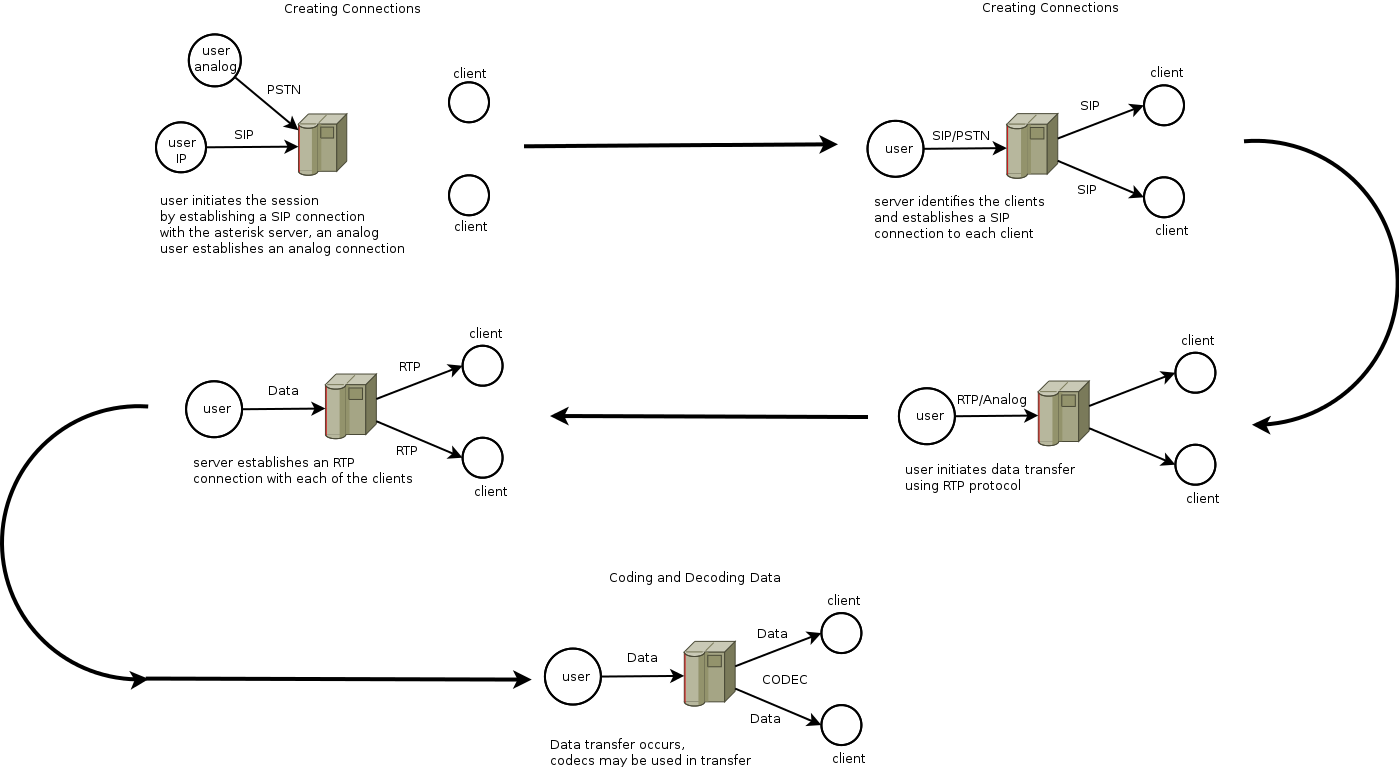
\includegraphics[width=\textwidth]{working.png}}
}
\subsection{Challenges}
\frame{
  \frametitle{Challenges}
  \begin{enumerate}
  \item Development of software for transmission and receiver.
  \item Development of a streamlined approach for configuring Asterisk PA System.
  \item Implementation and Testing.
  \end{enumerate}
}
\section{Prototype}
\subsection{Expenditure}
\frame[shrink,plain]{
  \frametitle{Expenditure}
  \begin{itemize}
  \item Consumables
    \begin{itemize}
    \item Network equipment Rs. 1500
    \item Import charges on equipment Rs. 7000
    \item Misc Charges: Rs. 1000

    \end{itemize}

  \item Equipment
    \begin{itemize}
    \item IP Phone  Rs. 5000
    \item IP speakers x2 Or Analog Gateway+ Speakers Rs. 10000
    \item Digium FXO cards - 1TDM410PLF Rs. 10000
    \end{itemize}
    
  \item Research Literature - Rs. 3000
  \item Others
    \begin{itemize}
    \item Uplink to telephony provider to test remote link. (college PBX)

    \end{itemize}

  \item Contingencies Rs. 1000.
    \begin{itemize}
    \item Rs. 4000 in case IP speakers are not available.

    \end{itemize}


  \end{itemize}
  {\bf Total Cost:} Rs.42500/-\\
  {\bf Real World Implementation:} Add cost of each client needed.
}

\section{Conclusion}          
\frame{
  \frametitle{Conclusion}
  \begin{enumerate}
   \item Only {\bf Open Source} Final Product in market.
   \item Provides easy and streamlined approach to install, configure and manage a system of any size - where as most proprietary system has a minimum limit.
   \item Uses open systems and protocols wherever possible.
   \item The system can be accessed remotely.
  \end{enumerate}
}
\end{document}

